% 2007 年四川卷文科第 6 题：题图。
% 来源 PDF：普通高考/2007/2007四川文.pdf，SHA256 1318df44733ec939e8789379d6fa2115a2c6a63e84b73c1f2bf3c080007ce68c
% 原页：第 1 页（A3 三栏）第 2 栏，印刷页 411，图在题干下方。
% 重绘依据：圆表示球（半径 2），A 为上极点，赤道画成水平椭圆，B 在左、C 在右；O 到 A、B、C 的半径虚线；与文科原页比对一致。
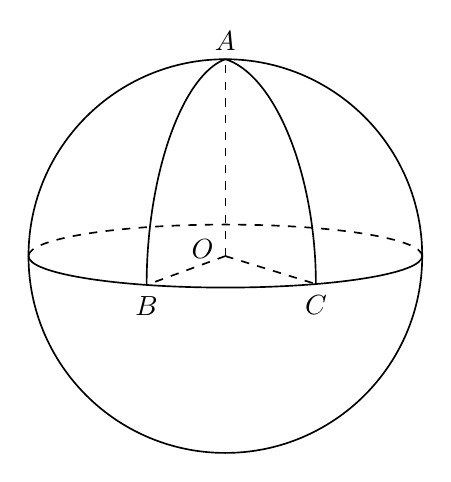
\begin{tikzpicture}[scale=1.25, semithick,
  every node/.style={inner sep=1.5pt}]
  % 球面轮廓与赤道
  \draw (0,0) circle (2);
  \draw[dashed] (2,0) arc[start angle=0, end angle=180, x radius=2, y radius=0.32];
  \draw (2,0) arc[start angle=0, end angle=-180, x radius=2, y radius=0.32];
  \coordinate (O) at (0,0);
  \coordinate (A) at (0,2);
  \coordinate (B) at (-0.800,-0.293);
  \coordinate (C) at (0.920,-0.284);
  % 球内半径（虚线）
  \draw[dashed] (O) -- (A);
  \draw[dashed] (O) -- (B);
  \draw[dashed] (O) -- (C);
  % 自 A 沿球面到 B、C 的经线弧（实线）
  \draw[domain=0:90, samples=80, smooth, variable=\t]
    plot ({2*sin(\t)*(-0.4000)},{2*cos(\t)+0.32*sin(\t)*(-0.9165)});
  \draw[domain=0:90, samples=80, smooth, variable=\t]
    plot ({2*sin(\t)*(0.4599)},{2*cos(\t)+0.32*sin(\t)*(-0.8881)});
  \node[anchor=south] at ([yshift=1pt]A) {$A$};
  \node[anchor=east] at ([xshift=-2pt,yshift=2pt]O) {$O$};
  \node[anchor=north] at ([yshift=-2pt]B) {$B$};
  \node[anchor=north] at ([yshift=-2pt]C) {$C$};
\end{tikzpicture}
